\documentclass[a4paper, 11pt, twocolumn]{article}
\usepackage[left=1.8cm, right=1.8cm, top=3cm, bottom=3cm]{geometry}
\setlength{\columnsep}{0.8cm}
\usepackage{booktabs}
\usepackage{graphicx}
\usepackage[activate={true,nocompatibility},final,tracking=true,kerning=true,spacing=true,factor=1100,stretch=10,shrink=10]{microtype}
\microtypecontext{spacing=nonfrench}
\usepackage{indentfirst}
\usepackage{notoccite}
\usepackage{listings}

\usepackage[croatian]{babel}
\usepackage[utf8]{inputenc}
\usepackage[T1]{fontenc}

% Učitaj pakete za kodnu stranicu 1250 i hrvatski jezik.
\RequirePackage{graphicx} % Uključeno jer je često korišteno
\RequirePackage{amssymb} % Uključeno jer je često korišteno
\RequirePackage{mathtools} % Uključeno jer je često korišteno
\RequirePackage[font={small, it}]{caption}
\RequirePackage{ifthen}
\RequirePackage{url} % Potrebno radi natbiba
\RequirePackage{enumitem} % Potrebno radi izmjene itemize okoline

% Ostali korisni paketi.
\RequirePackage{hyperref}
\RequirePackage{amssymb}
\RequirePackage{amsmath}

% Ovdje započinje članak.
\begin{document}

% Navedite naslov i autore. Datume se automatski postavlja na datum kreiranja dokumenta,
\date{15. siječnja 2017.}
\title{Harmonijska analiza glazbe korištenjem valićne transformacije} 
\author{Lovre Mrčela}
\maketitle

% Svako poglavlje započinje sa \section{Ime poglavlja} ako želimo da bude numerirano,
% a sa \section*{Ime poglavlja} ako ne želimo da bude numerirano.

\abstract{
U ovom radu provedena je harmonijska analiza glazbe upotrebom računala.
Harmonija u glazbi u najširem smislu podrazumijeva istovremeno zvučanje više tonova, te odnos među njima.
Pri analizi zvučnog signala korištena je valićna transformacija.

Svrha rada je omogućiti automatiziranu računalna obrada glazbenog isječka, u svrhu izvlačenja neke korisne informacije: tonaliteta, akorda ili pojedinih tonova melodije.
Svi navedeni postupci testirani su nad računalom generiranim glazbenim odsječcima u MIDI formatu, pretvorenima u Waveform Audio File format.
}

\section{Uvod}
Budući da je tema ovog rada glazba, u nastavku su objašnjeni neki osnovni glazbeni pojmovi koji su proučavani.
Također, pojašnjena je uloga valićne transformacije, te koji su problemi pri izvlačenju glazbenih tonova iz dobivene transformacije.

\subsection{Glazbeni pojmovi}
Pojednostavljeno govoreći, može se reći da je glazba niz tonova u vremenu proizvedenih na glazbenom instrumentu (uključujući i ljudski glas), gdje svaki ton ima svoju \textit{visinu}, \textit{trajanje}, \textit{glasnoću}, i \textit{boju}.
Jedan instrument, može proizvesti tonove različite visine, trajanja i glasnoće, dok svojstvo boje tona omogućuje razlikovanje instrumenata.
U užem smislu, pojam glazbenog tona se poistovjećuje sa njegovom visinom (npr. ton $c$).

Što se tiče sadržaja, glazba se može sastojati od istaknutih tonova koji čine melodiju, i pasivnih tonova koji čine pratnju toj melodiji; u tom slučaju radi se o \textit{homofonoj} glazbi.
Suprotno tome, glazba se može sastojati od više samostalnih melodija, i tada se radi o \textit{polifonoj} glazbi.

\textit{Harmonijska analiza} proučava vertikalnu strukturu glazbe: koji tonovi se čuju u određenom vremenskom trenutku, te koji je njihov međusoban odnos.
Za razliku od harmonijske, \textit{melodijska analiza} proučava horizontalnu strukturu glazbe: koji slijed tonova u vremenu čini melodiju, te koji je odnos između njih.
Dodatno, \textit{polifonijska analiza} je kombinacija dviju navedenih, te ona proučava kretanje više melodija istovremeno, i njihov odnos.
Ovaj rad bavi se harmonijskom, te u manjoj mjeri, melodijskom analizom.

Pojedini tonovi nazvani su slovima $a, h, c, d, e, f$, i $g$.
Ton povišen za pola označava se oznakom $\sharp$, a snižen za pola  oznakom $\flat$.
Razmaci između dvaju tonova su cijeli, osim između $h$ i $c$, te $e$ i $f$.
Unutar jedne oktave nalazi se 12 polutonova.
Radi jednostavnosti, u ovom radu oni su nazvani, redom $a, a\sharp, h, c, c\sharp, d, d\sharp, e, f, f\sharp, g,$ i $g\sharp$.

Na koncu, valja napomenuti da pojam \textit{akord} označava istovremeno zvučanje dvaju ili više tonova, te pojam tonalitet u najširem smislu podrazumijeva tonove od kojih je glazbeni isječak sastavljen.
Akord, odnosno tonalitet, pojednostavljeno govoreći, definiran je temeljnim tonom i ``vrstom''.
U ovom radu analizirat će se samo \textit{durska} i \textit{molska} ``vrsta'', koje se razlikuju po unutrašnjem rasporedu tonova.
Tako je npr. $C$-dur tonalitet (odnosno akord) definiran svojim temeljnim tonom $C$ i ostalim tonovima svojstvenima za raspored \textit{durske} ``vrste''\cite{osnove}.

\subsection{Uloga transformacije}
Format u kojem je glazba snimljena na računalu nije pogodan za detaljnu harmonijsku analizu, budući da se radi o ``spljoštenom'' jednodimenzionalnom signalu u vremenu.
Cilj valićne transformacije je ``izvući'' amplitudu signala na pojedinim frekvencijama, kako bi se iz nje mogli rekonstruirati snimljeni tonovi.

Amplitudno-frekvencijski sastav glazbenog tona u vremenu je složen.
Jedan glazbeni ton nije sastavljen od samo jedne frekvencije, niti jedna frekvencija u određenom vremenskom trenutku pripada nužno jednom tonu.
Naime, svojstvo boje tona glazbenog instrumenta uvjetuje pojavu dodatnih frekvencija, tzv. \textit{alikvota}, uz temeljnu frekvenciju koja je određena visinom tona.
Gledajući valićnu transformaciju, teško je odrediti koje frekvencije su temeljne, a koje određuju boju tona.
Ovaj problem detaljnije je opisan u potpoglavlju \ref{ss:alikvoti}.
Dodatno, u vremenskoj dimenziji jedan ton ravna se prema ADSR ovojnici, što otežava izdvajanje tona u vremenu.
Ovaj problem detaljnije je opisan u potpoglavlju \ref{ss:adsr}.

\section{Valićna analiza}
U ovom radu koristi se tzv. `bump' valić iz \textsc{Matlab}-ovog \textit{wavelet} paketa, čija Fourierova transformacija ima oblik\cite{matlab}:

$$ \Psi\left( a \omega \right) = \exp\left( 1 - \frac{1}{1 - \frac{\left(a \omega - \mu \right)^2}{\sigma^2}} \right)_{\left[ \frac{\mu - \sigma}{a}, \frac{\mu + \sigma}{a} \right]}, $$
gdje notacija $(\cdot)_{[a, b]}$ označava da je signal aktivan na području $[a, b]$, a van njega je jednak nuli.
Parametar $\mu$ određuje centar frekvencije valića i njegov dopušteni raspon je $[3, 6]$.
Parametar $\sigma$ određuje kompromis između vremenske i frekvencijske razlučivosti, i njegov dopušteni raspon je $[0.1, 1.2]$.

Parametar $\mu$ odabran je tako da pomnožen nekom potencijom broja 2 daje vrijednost 440\ Hz, prema kojoj se danas ugađaju instrumenti, a da je unutar dopuštenog raspona. Ta vrijednost je 3.4375.
Budući da je za primjenu ovog rada važnija veća preciznost u frekvencijama, parametar $\sigma$ postavljen je na minimalnu vrijednost, 0.1.

Korišteni raspon skala je takav da pokriva 88 tonova koji se mogu odsvirati na klaviru.
Taj raspon obuhvaća gotovo sve tonove koji se mogu odsvirati na današnjim standardnim instrumentima, od 27.5 Hz do 4186.01 Hz, uz korak s faktorom ${\frac{1}{12}}$ (12 tonova po oktavi).

Koristeći navedeni valić, ulazni glazbeni isječak transformira se kontinuiranom valićnom transformacijom u frekvencijskoj domeni.
Postupak transformacije je ovakav:
\begin{enumerate}
  \item DFT ulaznog glazbenog odsječka izračuna se korištenjem brze Fourierove transformacije,
  \item izračunavaju se funkcije valića za svaku zadanu skalu posebno, izravno u frekvencijskoj domeni,
  \item izračunavaju se umnošci pojedinog skaliranog valića sa DFT-om ulaznog glazbenog odsječka,
  \item IDFT-om nad svakim izračunatim umnoškom dobivaju se koeficijenti kontinuirane valićne transformacije.
\end{enumerate}

\section{Problemi u analizi}
U ovom dijelu opisani su prethodno navedeni problemi s \textit{alikvotima} i ADSR ovojnicom, te su navedeni načini kojima se njihov utjecaj može smanjiti prilikom određivanja glazbenih tonova iz transformacije.

\subsection{\textit{Alikvoti}}
\label{ss:alikvoti}
\textit{Alikvot} je pripadna frekvencija nekog glazbenog tona koja čini boju tona.
Kada u tonu ne bi bili sadržani \textit{alikvoti}, onda bi svi instrumenti imali jednaku boju tona.
Međutim, kod određivanja tona iz transformacije signala ovo zapravo stvara ``lažne frekvencije'' koje ne odgovaraju visinama stvarno odsviranih tonova.
Frekvencija $n$-tog \textit{alikvota} $f_n$ je višekratnik temeljne frekvencije tona $f_0$, odnosno $f_n = n \cdot f_0$.
Ovisno o načinu dobivanja tona u nekom instrumentu, \textit{alikvot} može nastati zbog rezoniranja kutije instrumenta, žica, stupca zraka, i sl.
Izgled transformacije s vidljivim \textit{alikvotima} prikazan je na slici \ref{fig:alikvoti}.

\begin{figure}[htb]
  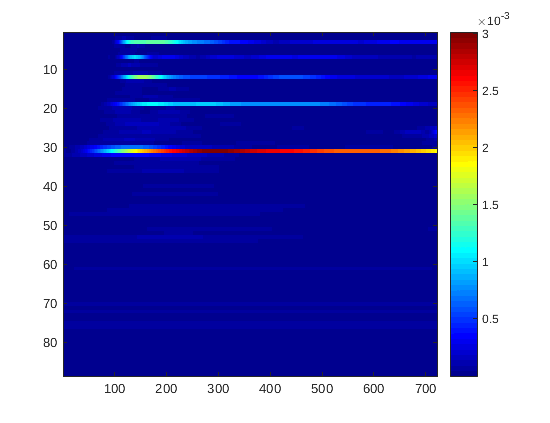
\includegraphics[width=\linewidth]{alikvoti}
  \caption{Rezultat transformacije glazbenog isječka koji ima odsviran samo jedan ton. Na x-osi prikazano je vrijeme, a na y-osi skala. Temeljna frekvencija prikazana je crvenom bojom, dok su frekvencije \textit{alikvota} udaljene za $\log_2{2}=1$ oktavu, $\log_2{3}=1.585$ oktava, $\log_2{4}=2$ oktave, $\log_2{5}=2.322$ oktava, itd. Alikvoti čija frekvencija nije ``pogođena'' skalom koja je korištena pri transformaciji izgledaju razmazano između dviju skala.}
  \label{fig:alikvoti}
\end{figure}

Također, neke od tih frekvencija mogu se preklapati sa visinama drugih tonova, te tako uzrokuju dodatno pojačanje osnovniih frekvencija.
Da stvar bude još gora, oni \textit{alikvotni} tonovi čija frekvencija nije faktor temeljne frekvencije i potencije broja 2 nisu ``pogođeni'' skalom korištenom pri transformaciji, pa one ubacuju smetnju čak i u više od jedne frekvencije istodobno.
Npr., frekvencija drugog alikvota je za $\log_2{3}=1.585$ oktava udaljena od temeljne frekvencija, što upada između dvije korištene skale, koje su udaljene za $\frac{19}{12}=1.583$ i $\frac{20}{12}=1.167$ oktava.

No, pokazalo se ipak da te smetnje nemaju velikog utjecaja na određivanje tonaliteta i akorda.
Naime, prva tri \textit{alikvota} nalaze se na frekvencijama udaljenima za jednu oktavu, kvintu iznad oktave (približno), i dvije oktave.
Kako je za određivanje tonaliteta ili akorda bitan samo naziv tona, oktave uopće ne smetaju budući da su to tonovi istog naziva, dok je što se tiče kvinte problem također nešto blaži budući da je neki akord uglavnom sadrži ton frekvencije kao što je ona.
Četvrti i viši \textit{alikvoti} uglavnom su preslabog intenziteta da bi pokvarili procjenu.

\subsection{ADSR ovojnica}
\label{ss:adsr}
ADSR (engl. \textit{Attack-Decay-Sustain-Release}) ovojnica je model generiranja glazbenog tona na \textit{synthesizerima} koja oponaša glazbeni instrument u stvarnom svijetu.
Četiri faze su: udar (engl. \textit{attack}), spust (engl. \textit{decay}), zadržavanje (engl. \textit{sustain}), i prigušivanje (engl. \textit{release}).
Ove četiri faze prikazane su na slici \ref{fig:adsr}.

\begin{figure}[htb]
  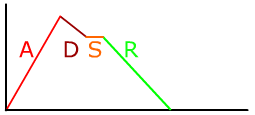
\includegraphics[width=\linewidth]{Adsr3}
  \caption{Shematski prikaz ADSR ovojnice, s naznačene četiri faze.}
  \label{fig:adsr}
\end{figure}

U fazi udara, ton naglo postiže maksimum glasnoće, što se čuje kao udar;
zatim se u fazi spusta glasnoća smanjuje do određene vrijednosti.
Ovo se događa kada instrument proizvede ton, npr. na pritisak tipke klavira, ili trzaj žice na gitari.
Nadalje, u fazi zadržavanja ton traje i stalne je glasnoće, a ovo odgovara držanju tipke na klaviru, ili prelaženju gudala preko žice uz konstantan pritisak i brzinu.
Na kraju u fazi prigušivanja, glasnoća opada i ton se više ne čuje, što odgovara otpuštanju tipke na klaviru, ili prigušenju žice na gitari prstima.

Odraz ovog efekta na izgled transformacije vidljiv je na slici \ref{fig:adsr_anomalija}.
Prilikom određivanja tonaliteta ili akorda glazbenog isječka, problem je u predugom trajanju signala u transformaciji, jer preklapanje ili nepreklapanje \\
pojedinih tonova u vremenu može navesti na krivi zaključak.

\begin{figure}[htb]
  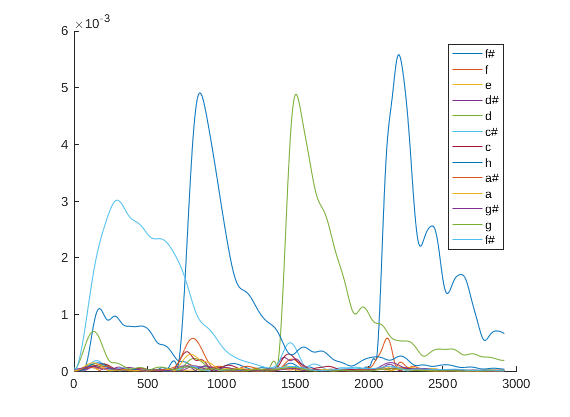
\includegraphics[width=\linewidth]{adsr_anomalija}
  \caption{Prikaz transformacija za 12 uzastopnih skala (jednu oktavu) na glazbenom isječku koji sadrži četiri uzastopno odsvirana tona ($f\sharp, h, d, f\sharp$). Svaki ton prikazan je različitom bojom. Za svaki ton vidljiv je oblik ADSR ovojnice. Uočljiva je i pojava \textit{alikvotne} frekvencije u prvom odsviranom tonu: to je ujedno i osnovna frekvencija četvrtog odsviranog tona.}
  \label{fig:adsr_anomalija}
\end{figure}

Predloženo rješenje ovog problema je promatranje derivacije transformacije po vremenskoj komponenti.
Maksimum derivacije pokazuje gdje glasnoća tona najbrže raste, a to je upravo u prvoj fazi ADSR ovojnice.
Derivirani signal prikazan je na slici \ref{fig:adsr_der}.
Time se lakše može odrediti pozicija tonova koji sviraju istovremeno.

\begin{figure}[htb]
  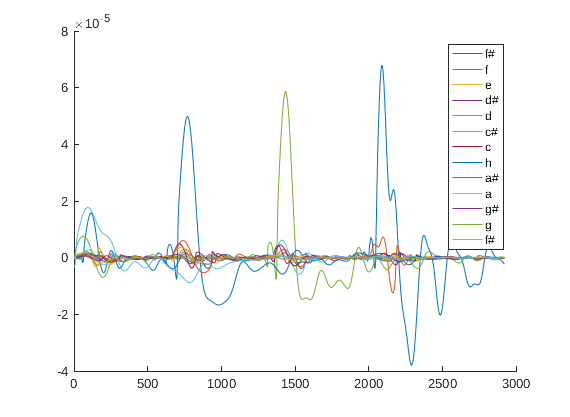
\includegraphics[width=\linewidth]{adsr_der}
  \caption{Derivacija prethodno prikazane transformacije po vremenu. Udari tonova sad su kompaktno smješteni.}
  \label{fig:adsr_der}
\end{figure}

\section{Ekstrakcija informacija}
U ovom dijelu ukratko su opisani postupci dobivanja željene informacije.
Ekstrakcija informacija obavlja se na prethodno dobivenoj valićnoj transformaciji.

\subsection{Tonalitet}
Analiza tonaliteta na temelju glazbenog isječka provodi se na sljedeći način:
\begin{enumerate}
  \item za svaku skalu izračuna se vremenski prosjek intenziteta,
  \item prag se odredi kao ukupan prosjek po svim skalama,
  \item odbacuju se one skale koje su ispod praga,
  \item preostale skale se prevode u nazive tonova čije su to temeljne frekvencije,
  \item usporedbom sa strukturom nekog tonaliteta odabire se onaj tonalitet kojemu dobivene skale najviše odgovaraju.
\end{enumerate}

\subsection{Akord}
Analiza akorda u glazbenom isječku provodi se na sljedeći način:
\begin{enumerate}
  \item pretraživanjem derivacije transformacije po vremenu određuju se mjesta na kojima sviraju barem 3 tona istovremeno (ne brojeći \textit{alikvote})
  \item slično analizi tonaliteta, analizira se tonski sastav, i odbacuju one skale koje su ispod praga,
  \item preostale skale se prevode u nazive tonova čije su to temeljne frekvencije,
  \item usporedbom sa strukturom nekog akorda i bira se onaj kojemu dobivene skale najviše odgovaraju.
\end{enumerate}

\subsection{Melodija}
Analiza melodije najjednostavniji je primjer. Provodi se na sljedeći način:
\begin{enumerate}
  \item pretraživanjem derivacije transformacije po vremenu određuju se mjesta na kojima tonovi započinju svirati,
  \item uzima se najveća skala u tim trenutcima, te se prevodi u nazive tonova.
\end{enumerate}

\section{Zaključak}
U ovom radu prikazan je praktičan postupak ekstrakcije informacije o tonalitetu, akordima, ili melodiji iz glazbenog isječka koristeći pritom `bump' valić i izračun u frekvencijskom području.
Pojavljuju se dvije vrste problema s određivanjem tonova iz dobivene transformacije.
Problemi zbog \textit{alikvota} su zanemareni zbog oslanjanja na robusnost samih postupaka za ekstrakciju informacija.
Problem razmazivanja u vremenu riješen je na način da se početci tonova uzimaju kao mjesta gdje je derivacija transformacije maksimalna, odnosno tonovi najbrže povećavaju glasnoću, kako bi se moglo odrediti koji tonovi sviraju skupa.

Detaljnijom analizom oblika \textit{alikvota} za svaki instrument, moglo bi se poboljšati njihovo uklanjanje prilikom obrade glazbenog isječka.
Iako se oni mogu zanemariti u računalom generiranim primjerima, kod snimaka glazbe iz stvarnog svijeta njihov utjecaj nije zanemariv.

\begin{thebibliography}{25}
\bibitem{osnove}
Tihomir~Petrović,
Osnove teorije glazbe.
2010.

\bibitem{matlab}
Continous wavelet transform using FFT algorithm.
URL: https://www.mathworks.com/\\help/wavelet/ref/cwtft.html

\end{thebibliography} 
\end{document} 